\section{Methods}\label{sec:methods}

\subsection{Features}
From the raw tables we construct \nFeatures{} features in eight groups (Table~\ref{tab:features}). Weather and satellite variables are aggregated by growth stage (sums for rain; means, minima and maxima for moisture, temperature and indices) and complemented by season metrics: total rain and its anomaly relative to the district's previous seasons, the number of dry and hot months, growing degree-days (base 10\,$^\circ$C), vapour-pressure deficit, and the NDVI peak, area, timing and green-up rate after linear gap-filling of cloud-missing months, together with a clear-sky fraction. Price features convert lag-1 national prices into local farm-gate prices; price ratios and a log competing-revenue index summarise relative profitability. Map features include distances, irrigated and paddy shares, flood frequency and $k$-nearest-neighbour ($k=8$) spatial lags of the neighbours' previous-season yields and current-season NDVI anomalies.

Four rules make the features leakage-safe: (i) yield history uses previous seasons only; (ii) prices are lagged one season; (iii) weather and satellite data are truncated at the forecast cut-off month; and (iv) anomalies are computed against each district's previous seasons. The rules are enforced by automated tests that perturb all data of later seasons and verify that the features of earlier seasons are unchanged, and---as a check of the test itself---that each deliberately leaky variant of Section~\ref{sec:leakmethods} fails it.

\begin{table}[t]\centering\scriptsize
\caption{Feature groups, number of features, content, and the real-data sources that can replace the synthetic inputs without code changes (OAE: Office of Agricultural Economics; DOAE: Department of Agricultural Extension; TMD: Thai Meteorological Department; RID: Royal Irrigation Department; OCSB: Office of the Cane and Sugar Board; LDD: Land Development Department; GISTDA: Geo-Informatics and Space Technology Development Agency).}\label{tab:features}
\begin{tabularx}{\textwidth}{@{}p{3.3cm}cXp{3.4cm}@{}}
\toprule
Group & $n$ & Features & Real-data sources \\
\midrule
Previous yields & 5 & lags $t-1$, $t-2$; previous-3-season mean and s.d.; 5-season trend & OAE / DOAE statistics \\
Humidity \& soil moisture & 12 & RH, VPD, soil-moisture mean and minimum per growth stage & ERA5-Land; SMAP \\
Water (rain, reservoir, irrigation) & 8 & rain per stage and season; anomaly vs. past; dry months; reservoir storage; irrigation supply & CHIRPS; TMD; RID reservoirs \\
Climate (temperature, GDD) & 9 & $T_{\mathrm{mean}}$, $T_{\max}$ per stage; GDD; hot months; rainfall normal & ERA5-Land; TMD normals \\
Satellite (NDVI, EVI, LSWI, LST) & 19 & NDVI/EVI maxima, LSWI/LST means per stage; NDVI peak, area, timing, green-up; clear-sky fraction; anomalies & MODIS MOD13Q1, MOD09A1, MOD11A2; Sentinel-1/2 \\
Prices (own \& competing crops) & 11 & lag-1 local prices of rice, cassava, sugarcane, maize; ratios; competing-revenue index; rice/urea ratio & OAE farm-gate prices; OCSB cane price \\
Geography (terrain, soil) & 9 & elevation, slope, sand, SOC, pH, saline share, suitability class, coordinates & SRTM; LDD soil maps; SoilGrids \\
Map layers \& spatial lags & 8 & distances to river, mill and market; irrigated and paddy share; flood frequency; $k$-NN spatial lags & RID; LDD land use; GISTDA floods; OSM \\
\midrule Total & 81 & & \\
\bottomrule
\end{tabularx}
\end{table}

\subsection{Learners}
We compare eight learners of increasing flexibility. \emph{Persistence} forecasts last season's yield and \emph{climatology} the mean of the previous three seasons, $\bar y^{(3)}_{it}$. The \emph{panel fixed-effects} (FE) model is the econometric baseline: a within estimator with district effects, a linear trend and all time-varying covariates, with lagged yields excluded to avoid dynamic-panel bias and a small ridge penalty for numerical stability \citep{wooldridge2010econometric}. \emph{Ridge regression} \citep{hoerl1970ridge} uses standardised, median-imputed features with the penalty chosen by efficient leave-one-out cross-validation within the training data. The \emph{random forest} \citep{breiman2001random} has 200 trees. The \emph{multilayer perceptron} (MLP; hidden layers of 64 and 32 units, early stopping) represents neural approaches. \emph{LightGBM} \citep{ke2017lightgbm} is a histogram-based gradient-boosting machine that handles missing values natively. The \emph{ensemble} averages LightGBM and Ridge with equal weights, combining the threshold-and-interaction capacity of trees with the smooth extrapolation of a linear model; fixed weights avoid an additional layer of fitting \citep[cf.][]{wolpert1992stacked}.

Two target formulations are considered: the yield level $y_{it}$, and the anomaly $y_{it}-\bar y^{(3)}_{it}$, which removes district effects and slow trends that trees cannot extrapolate; anomaly forecasts are added back to $\bar y^{(3)}_{it}$.

\subsection{Validation protocol}
All evaluation uses a rolling origin \citep{tashman2000out}: the forecast for season $t$ comes from a model fitted on seasons $s<t$ only. Seasons 2008--2010 serve only to initialise lagged features. LightGBM hyper-parameters and the target formulation are tuned jointly by random search (\nTrials{} configurations $\times$ 2 targets) on the validation seasons 2015--2017, each forecast with rolling origin, and the main model is then selected among LightGBM, Ridge and the ensemble on the same validation seasons. The test seasons 2018--2025 (8 seasons $\times$ \nDistricts{} districts $=1{,}600$ forecasts) were used only after all choices had been frozen.

\subsection{Performance measures and inference}\label{sec:metrics}
We report RMSE, MAE, MAPE and the coefficient of determination $R^2$, together with two skill measures that are not inflated by the large between-district variance:
\begin{equation}\label{eq:skill}
R^2_{\mathrm{anom}} = 1-\frac{\sum_{it}(y_{it}-\hat y_{it})^2}{\sum_{it}(a_{it}-\bar a)^2},\qquad
\mathrm{Skill} = 1-\frac{\mathrm{MSE}}{\mathrm{MSE}_{\mathrm{clim}}},\qquad a_{it}=y_{it}-\bar y^{(3)}_{it}.
\end{equation}
$R^2_{\mathrm{anom}}$ is the share of the deviation from the recent mean that is predicted, and Skill is the reduction of the climatology's mean squared error. Because errors are strongly correlated within seasons, uncertainty is quantified with a season-block bootstrap that resamples whole test seasons \citep{kunsch1989jackknife,efron1993introduction} ($B=2{,}000$). Accuracy differences relative to the main model are tested with the Diebold--Mariano test \citep{diebold1995comparing} applied to the season-level differentials $d_t$ of mean squared errors, with the correction of \citet{harvey1997testing} for $T=8$ one-step-ahead forecasts,
\begin{equation}\label{eq:dm}
\mathrm{DM}^{*}=\sqrt{\frac{T-1}{T}}\;\frac{\bar d}{\sqrt{\hat\gamma_0/T}}\ \sim\ t_{T-1},
\end{equation}
where $\hat\gamma_0$ is the sample variance of $d_t$; $p$-values are adjusted with the Holm procedure \citep{holm1979simple}.

\subsection{Leakage audit (E2)}\label{sec:leakmethods}
LightGBM, Ridge and the ensemble are re-estimated under four flawed protocols and scored on the same 1{,}600 test forecasts: (i) random 5-fold cross-validation over all district-seasons, which trains on future seasons and same-season neighbours; (ii) same-season instead of lag-1 prices; (iii) an additional spatial lag of neighbours' current-season yields; and (iv) weather and NDVI anomalies computed against the full-period district mean. Optimism is expressed as the relative reduction of RMSE compared with the leakage-safe protocol.

\subsection{Attribution and ground-truth recovery (E3--E4)}
Predictive value is measured by drop-one-group ablation: each group is removed, the model is re-trained in every fold and the RMSE change is computed with season-bootstrap intervals. When the history group is removed, the level target is used, because the anomaly target presupposes past yields. Attributions are computed for every test forecast: TreeSHAP for LightGBM \citep{lundberg2020local} and exact linear SHAP, $\phi_j=\beta_j(x_j-\mathbb E x_j)$, for Ridge; because Shapley values are additive in the model output, the ensemble's attribution is the average of the two. Group attributions are sums, $\Phi_G=\sum_{j\in G}\phi_j$. Ground-truth recovery is assessed by the Pearson correlation between each true component of Eq.~\eqref{eq:yield} and $\Phi_G$ for every group, and by comparing binned SHAP dependence curves with the binned true component along the main observed driver.

\subsection{In-season forecasting (E5)}
Features are rebuilt with data cut-offs at the end of July, August, September, October and November, and the full protocol is repeated with and without the satellite group. The difference measures the marginal value of satellite data at each forecast date.

\subsection{Prediction intervals (E6)}
Prediction intervals use rolling split-conformal calibration: for test season $t$, the interval is $[\hat y_{it}+q_{\alpha/2},\ \hat y_{it}+q_{1-\alpha/2}]$, where $q$ are empirical quantiles of the main model's out-of-sample errors in all earlier seasons from 2014 onwards. This respects the forecasting information set. We evaluate 80\% and 90\% intervals overall, by season, and separately in \emph{shock seasons}, defined as seasons whose regional mean anomaly $\bar a_t$ lies more than one standard deviation below the mean of all seasons.

\subsection{Robustness (E7)}\label{sec:robustness}
The tuned configuration is applied without re-tuning to ten independently simulated replicate worlds (seeds 1000--1009) and to the four scenario worlds. For each world we record the RMSE of climatology, Ridge, LightGBM and the ensemble, of the ensemble without satellite features, and of the ensemble scored by random cross-validation.

\subsection{Implementation and reproducibility}
The pipeline is written in Python~3.12 with NumPy, pandas, scikit-learn \citep{pedregosa2011scikit} and LightGBM~4.7, and the complete set of experiments runs on a single CPU core in about \runMinutes{} minutes. Every number in this paper is written to a macro file by code from saved results. Raw inputs follow a documented schema; a Google Earth Engine script extracts their real counterparts (MODIS vegetation indices, LSWI and LST, CHIRPS rainfall, ERA5-Land weather and soil moisture, SRTM terrain and a cropland mask) for any set of district polygons (Table~\ref{tab:features}). Maps are drawn with GeoPandas from Natural Earth boundaries \citep{naturalearth} by \texttt{thailand\_map.py}.

\begin{figure}[t]\centering
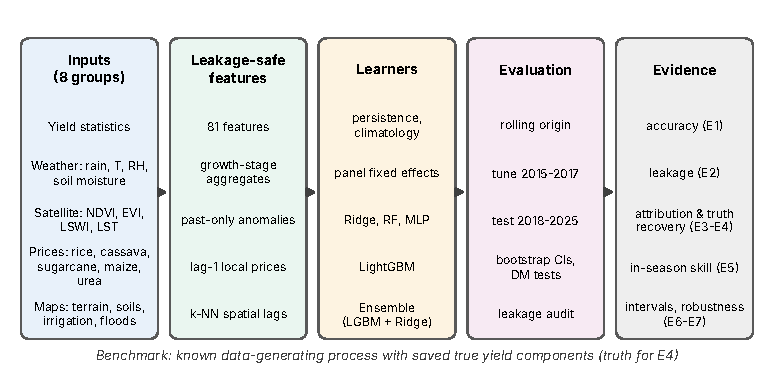
\includegraphics[width=\textwidth]{fig2_workflow}
\caption{Study workflow: inputs in eight groups are turned into leakage-safe features, eight learners are evaluated with a rolling origin, and seven experiments (E1--E7) provide the evidence for RQ1--RQ4. The simulator's stored true yield components enable the ground-truth test of explanations (E4).}\label{fig:workflow}
\end{figure}
